\documentclass[addpoints]{exam}

\usepackage{graphbox}
\usepackage{hyperref}
\usepackage{listings}
\usepackage{subcaption}
\usepackage{tabularx}
\usepackage{tikz}
\usetikzlibrary{positioning}

% Header and footer.
\pagestyle{headandfoot}
\runningheadrule
\runningfootrule
\runningheader{CS 440}{HW 3: Meshes and Transformations}{Fall 2023}
\runningfooter{}{Page \thepage\ of \numpages}{}
\firstpageheader{}{}{}

% \qformat{{\large\bf \thequestion. \thequestiontitle}\hfill[\totalpoints\ points]}
\qformat{{\large\bf \thequestion. \thequestiontitle}\hfill}
\boxedpoints

\title{Homework 3: Meshes and Transformations}
\author{CS 440 Computer Graphics\\Habib University}
\date{Fall 2023}

\begin{document}
\maketitle

Each problem below specifies the names of the files that you have to submit for it. Please make sure that your submitted files have the indicated names. Any files in your GitHub repository with these names at the time of the deadline will be considered your submission.

\begin{questions}

  \titledquestion{A repository of models}

  \begin{tabularx}{\linewidth}{lX}
    \raisebox{-.95\totalheight}{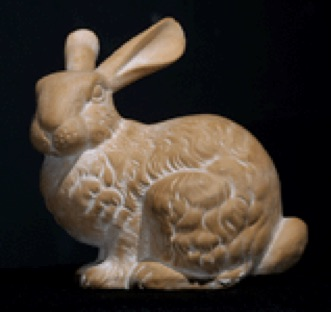
\includegraphics[width=.3\textwidth]{bunny}}
    &
      Obtain some models from the \href{http://graphics.stanford.edu/data/3Dscanrep/}{The Stanford 3D Scanning Repository} to work with. You will need to run a local web server, as in the previous homework, to load the file into your program and perform the following operations.
      
Include interface elements to support the following GPU operations on the loaded model.
\end{tabularx}
  \begin{parts}
  \part On the CPU, read in the geometry and compute its bounding box. Send the bounding box information as a \texttt{uniform} to the vertex shader which then transforms the vertices to clip coordinates such that the aspect ratio of the model is preserved, the model is centered at the origin, and it is fully visible. Use \href{https://webgl2fundamentals.org/webgl/lessons/webgl-indexed-vertices.html}{indexed vertices} to minimize the number of vertices that need to be passed to the GPU.
  \part Rotate the model slightly about each of the 3 axes in the clockwise or counterclockwise direction.
  \part Shift the model slightly in the positive or negative x, y, or z directions.
  \part Scale the model slightly along any of the x, y, or z directions.
  \part Reflect the model about any of the axes.
  \part Reset all transformations.
  \end{parts}

  The model may appear flat. Try to use \href{https://registry.khronos.org/OpenGL-Refpages/gl4/html/gl_FragDepth.xhtml}{gl\_FragDepth} to create a perception of depth.

  \underline{Files}: {\tt mesh.html, mesh.js}

\end{questions}

\end{document}

%%% Local Variables:
%%% mode: latex
%%% TeX-master: t
%%% End:
